Development of DoS started with development in phases which focus on particular need of project.
Various phases and their detail are given below -:
\begin{itemize}
\item Phase I (Sagemath) -: \\
	During Phase I, we wrote code in Sagemath to compute all the required output variable.
We used two files for this.Input variable are written in input.sage and main.sage loads this variable and 
compute all desired inputs.
\item Phase II (\LaTeX{}) -: \\
	During phase II, we embedded sage modules into \LaTeX{} by loading them into civil.tex and then displayed these
	variables in output PDF and all this work is done by sagetex.sty. To execute all this commands on one go 
	we wrote script civil.sh.
\item Phase III (Django) -: \\
	During phase III, we provided web interface to this software using Django. Djanog was used
	to get input from user and write input.sage file for particular user then civil.sh 
	is called by passing name of user directory to it and then get output PDF.
\item Phase IV (Improvise) -: \\
	During phase IV, we improved the code structure and added additional 
	functionality like sending PDF as email and accepting input as CSV file.
	Finally, the UI was improved and made responsive.
\item Phase V (Testing) -: \\
During phase V, we tested the software for various conditions and then applied required error control and messaging 
mechanism. initialfile.py file was created to save software from problem of server restart which can causes processing user request to stop. so, that 
the interrupted request of user can be restart and send PDF.
\item Phase VI (Documentation) -: \\ 
During final phase, we documented the project( developers documentation and README.md) using doxygen and wrote the report for this software.    
\end{itemize}     

\begin{figure}[H] 
\centering 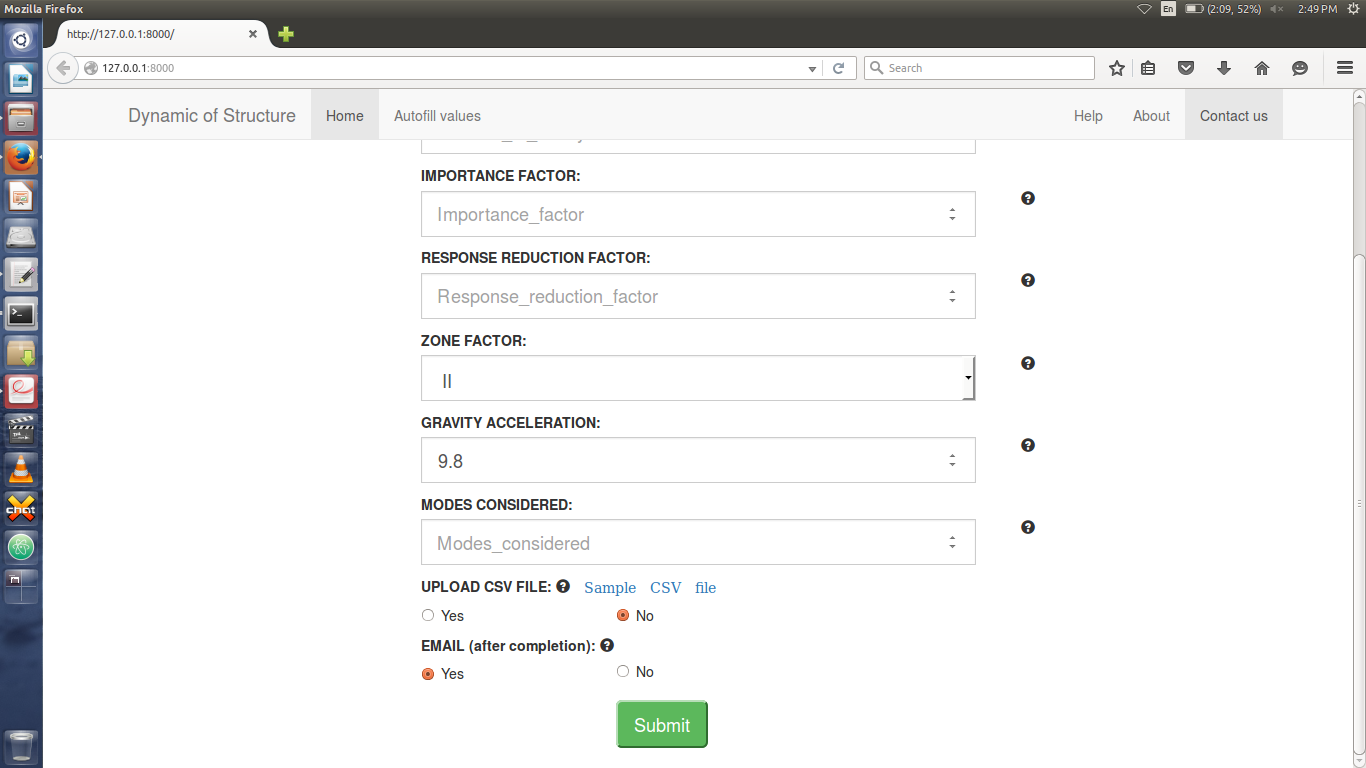
\includegraphics[scale=0.32]{images/output/1.png}
\caption{Home page of DoS}
\label{fig:1}
\end{figure}
This is the first interface that is shown to the user. This is the Home page.
It brings a nice UI to get input from user about the Number of storeys and 
some factor affecting the structure. It also provides the user some 
additional features as an aid like uploading data as CSV files and Email 
after completion. There is an additional help icon near every field to get 
an idea of what it is. There is a static navigation bar that provides an 
Auto fill values option. By clicking that option, default values are 
automatically filled figure \ref{fig:1} and figure \ref{fig:9}.
\begin{figure}[H] 
\centering 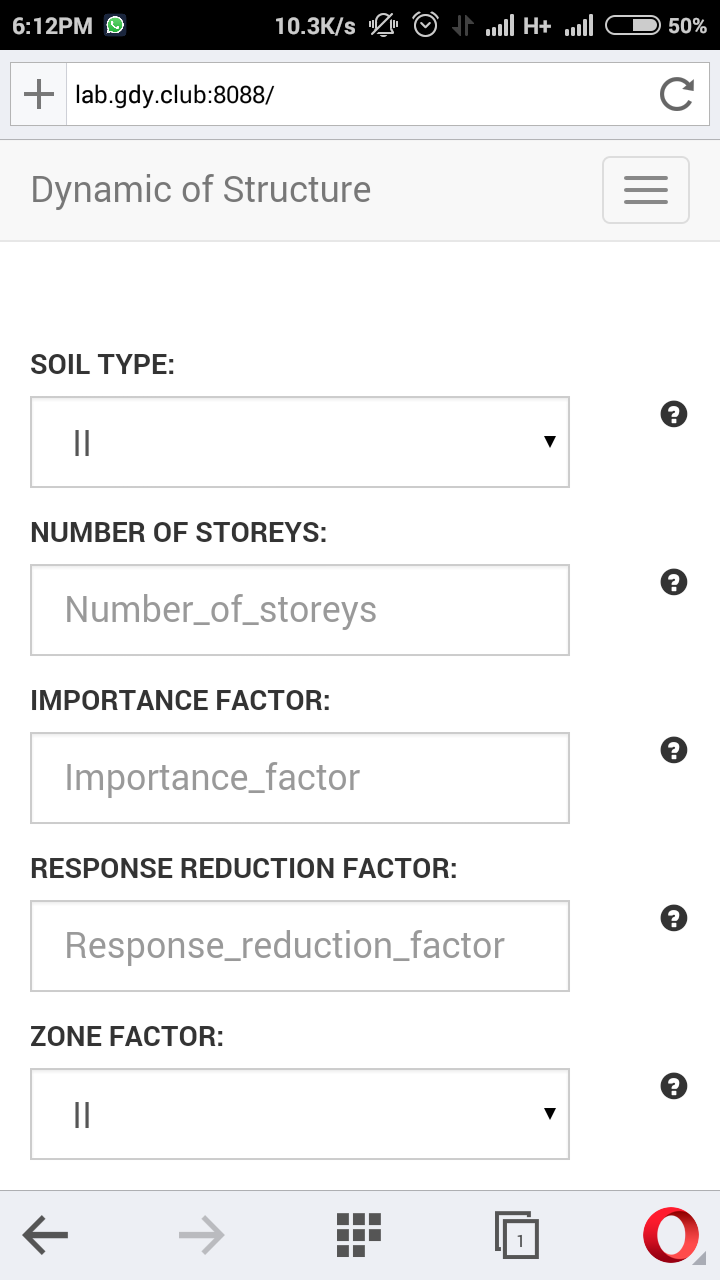
\includegraphics[scale=0.32]{images/output/5.png}
\caption{Home page of DoS(mobile view)}
\label{fig:9}
\end{figure}  


After clicking the 'Submit' button on the homepage, user is shown another 
form based on his input "Number of Storeys" in the homepage form, for 
filling out the matrix values manually Figure \ref{fig:2}.

\begin{figure}[H] 
\centering 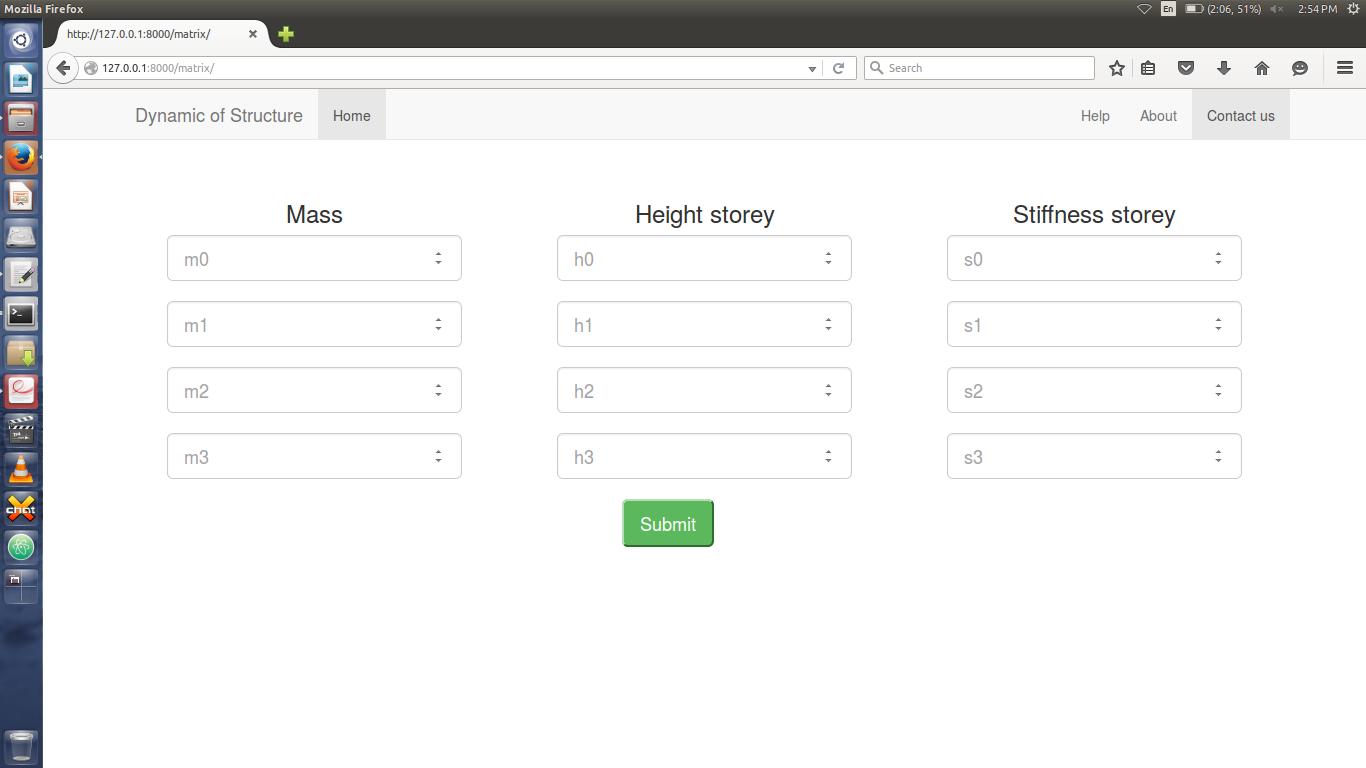
\includegraphics[scale=0.32]{images/output/2.png}
\caption{Matrix.html for manually filling values}
\label{fig:2}
\end{figure}

The top navigation bar is static to all pages. There is a link to the Help. 
After clicking which, the help regarding the different inputs fields 
provided Figure \ref{fig:3}.

\begin{figure}[H] 
\centering 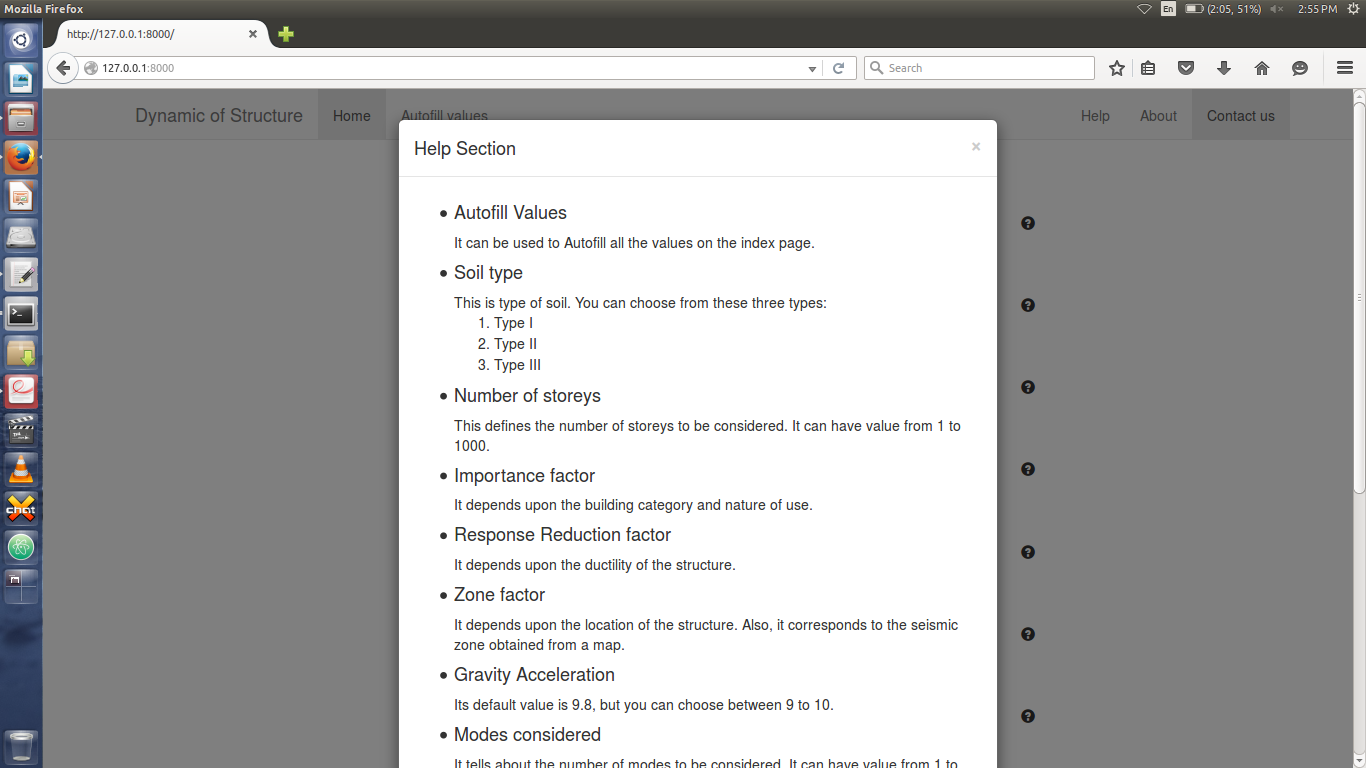
\includegraphics[scale=0.31]{images/output/3.png}
\caption{Help section in Home page}
\label{fig:3}
\end{figure}

There are small icons near each of the input field on the homepage. They are 
the help icons. After hovering them, they display a little help related to
that correspond field Figure \ref{fig:4}.
\begin{figure}[H] 
\centering 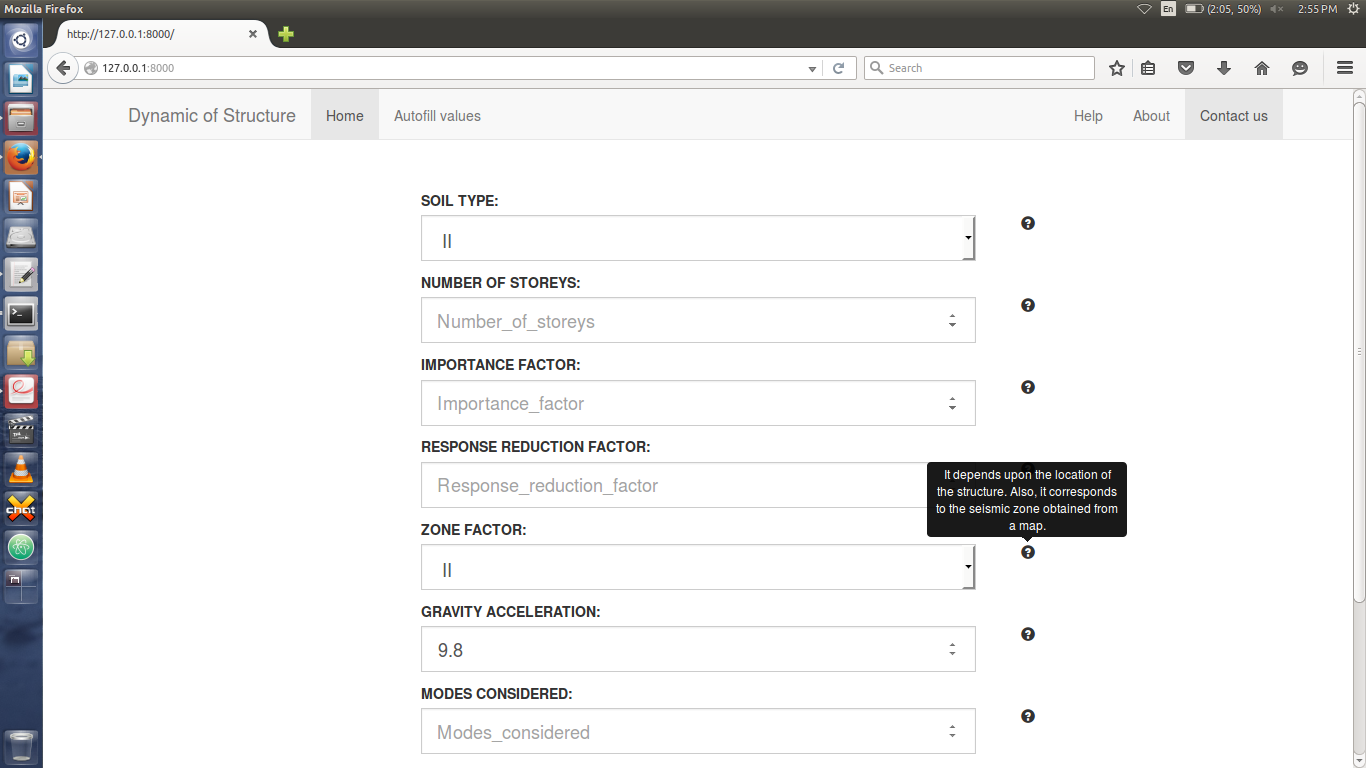
\includegraphics[scale=0.31]{images/output/4.png}
\caption{Local help option}
\label{fig:4}
\end{figure}

After running a set of commands of \LaTeX and SageMath, it produces the
output in PDF form (with pdflatex) Figure \ref{fig:5}.
\begin{figure}[H] 
\centering 
\includegraphics[scale=0.31]{images/output/6.png}
\caption{First page of PDF generated by DoS}
\label{fig:5}
\end{figure}

After the titlepage, table of content and some other stuff, the PDF contains 
the values (matrices) entered in the form at the homepage Figure \ref{fig:6}.
\begin{figure}[H] 
\centering 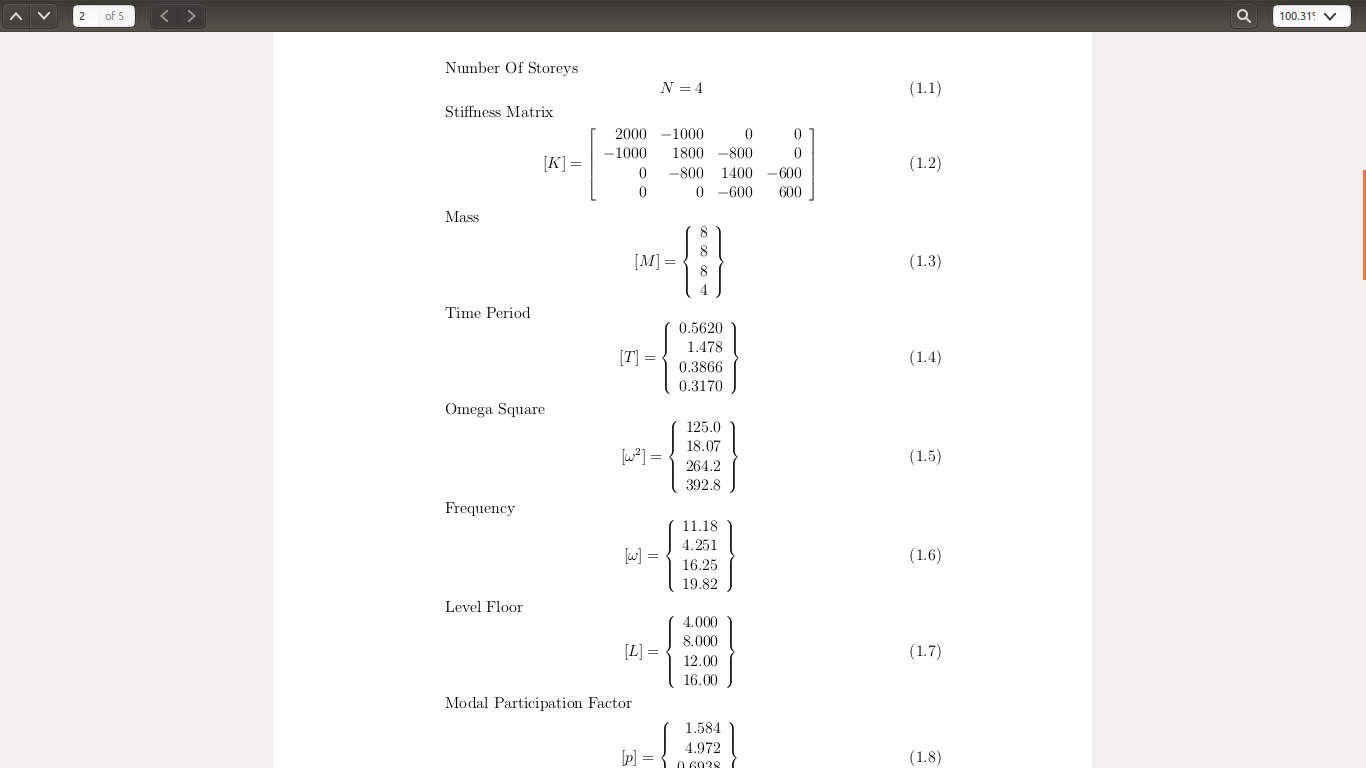
\includegraphics[scale=0.31]{images/output/7.png}
\caption{Initial values given for checking in PDF}
\label{fig:6}
\end{figure}

There is graph embedded in the PDF which is being created using Sagemath Figure \ref{fig:7}.
\begin{figure}[H] 
\centering 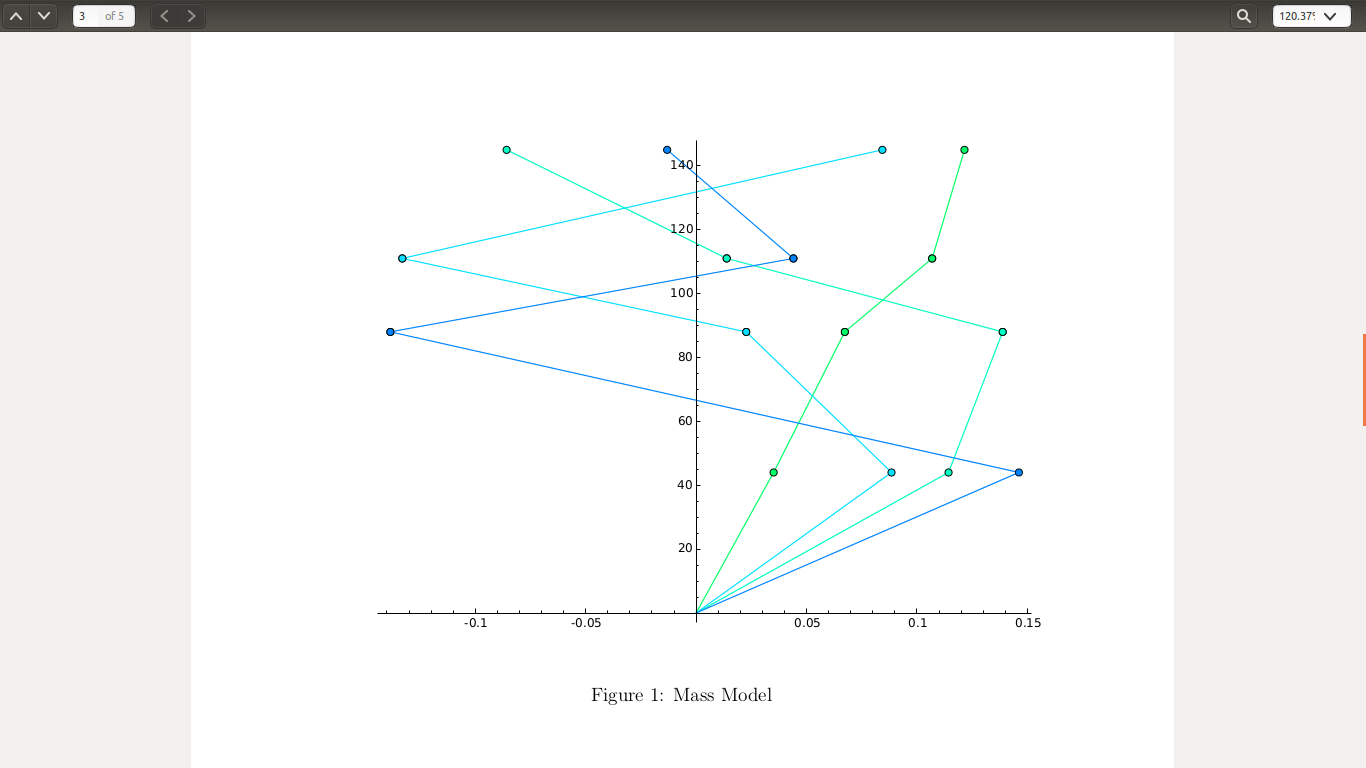
\includegraphics[scale=0.31]{images/output/8.png}
\caption{Graph Generated in PDF}
\label{fig:7}
\end{figure}

After all calculations, the computed final result is printed on the PDF Figure \ref{fig:8}.
\begin{figure}[H] 
\centering 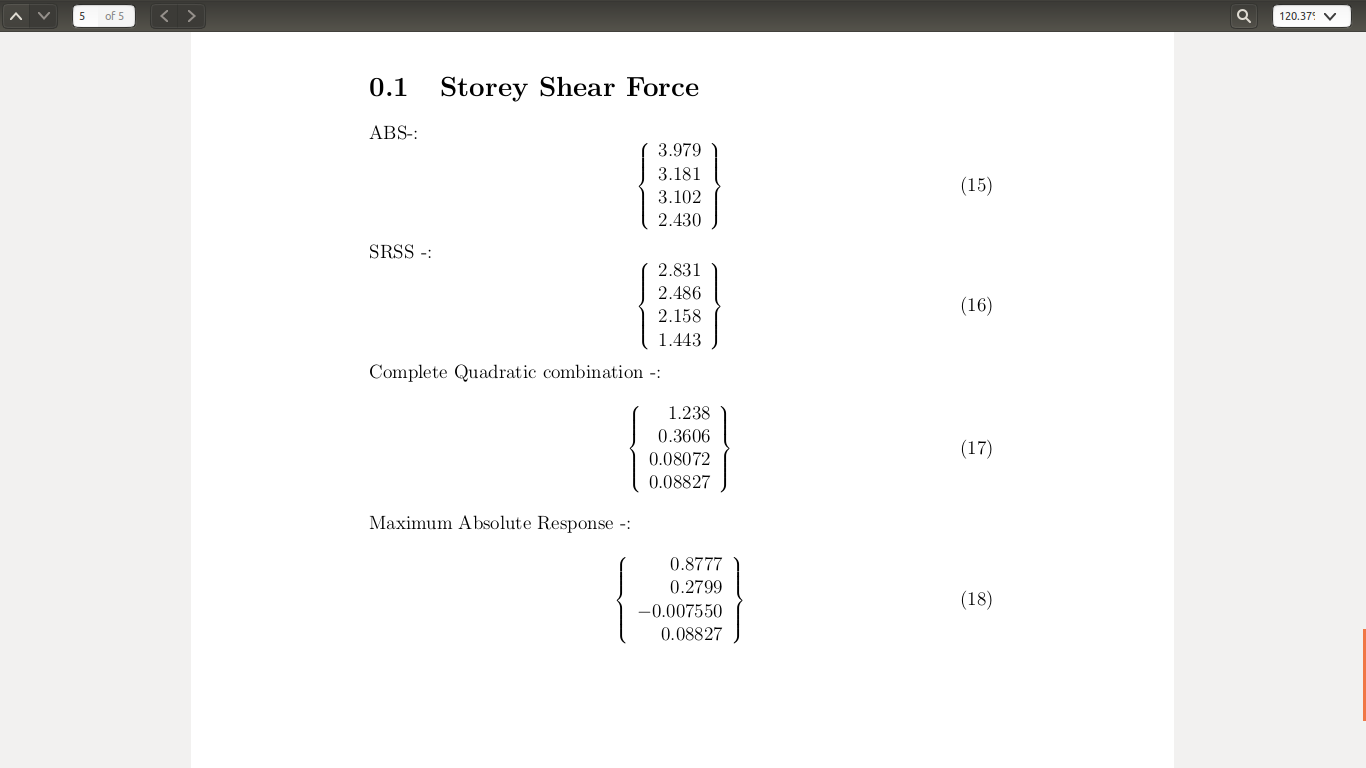
\includegraphics[scale=0.31]{images/output/9.png}
\caption{Final output in PDF}
\label{fig:8}
\end{figure}
